\documentclass[11pt]{article}
\usepackage[T1]{fontenc}
\usepackage[utf8]{inputenc}
\usepackage{lmodern,amsmath,amssymb,amsthm,mathtools,booktabs,enumitem,microtype,longtable,array,tikz}
\usepackage[margin=1in]{geometry}
\usepackage[colorlinks=true,linkcolor=blue,urlcolor=blue,citecolor=blue]{hyperref}
\hypersetup{pdftitle={Finite Instructions and Solenoidal Shear Flows},pdfauthor={OpenAI}}
\newtheorem{theorem}{Theorem}[section]
\newtheorem{lemma}[theorem]{Lemma}
\newtheorem{corollary}[theorem]{Corollary}
\newtheorem{proposition}[theorem]{Proposition}
\newtheorem{definition}[theorem]{Definition}
\theoremstyle{remark}
\newtheorem{remark}[theorem]{Remark}
\newcommand{\T}{\mathbb T}
\newcommand{\Z}{\mathbb Z}
\newcommand{\N}{\mathbb N}
\newcommand{\R}{\mathbb R}
\newcommand{\Q}{\mathbb Q}
\newcommand{\diag}{\operatorname{diag}}
\newcommand{\supp}{\operatorname{supp}}
\newcommand{\divg}{\operatorname{div}}
\newcommand{\id}{\operatorname{id}}
\title{Finite Instructions and Solenoidal Shear Flows}
\author{OpenAI}
\date{September 27, 2026}
\begin{document}
\maketitle
\begin{abstract}
We realize finite reciprocal affine instruction maps by smooth incompressible
shear flows on a flat three-torus. Applied to a reversible one-head recorder
with a finite transition table, this gives a complete machine-to-fluid construction:
a fixed particle enters a fixed open strip exactly when a given machine halts,
with zero initial velocity, zero pressure, and a solenoidal mean-zero force
that is periodic after initialization. The construction acts on full closed
rectangles and controls every intermediate trajectory. Separate heights
resolve overlap between sources and targets, and an endpoint-size estimate
controls all excursions independently of the reciprocal scaling factor.
\end{abstract}

\section{From finite instructions to a fluid experiment}\label{sec:intro}
A local machine instruction changes finitely many symbols, but its smooth
realization must move every nearby point consistently. There are two obstacles.
An irreversible instruction may merge distinct inputs, whereas a smooth flow
has an injective time map. Even after the instruction is made reversible,
a source rectangle can overlap another instruction's destination. The first
obstacle asks for retained history; the second asks for an order of geometric
operations that does not disturb data waiting to move.

Information retention is the classical basis of reversible simulation.
Landauer discusses its logical role \cite[Section~3]{Landauer}, and Bennett
records the index of the instruction just performed on a history tape
\cite[Eqs.~(9)--(11)]{Bennett}. We use that principle in a one-head
recorder with a finite transition table, a moving history frontier, and a
temporary return mark. We prove the full-domain inverse of our particular
local table explicitly. Moore's generalized shifts \cite{Moore} provide the
positional-coding viewpoint: tape prefixes become separated real intervals,
and head moves become affine expansions and contractions. Here the exact
closed rectangles, their gaps, and the entire continuous motion are also
part of the argument.

Fluid realizations of computation have a geometric history as well.
Cardona, Miranda, Peralta-Salas and Presas construct stationary Euler
computation on an adapted Riemannian three-sphere, using an area-preserving
realization of generalized shifts \cite{CMPP}. Their neighborhood contraction,
transport, and expansion in Proposition~5.1 is a related geometric predecessor.
For the Euclidean metric, Cardona, Miranda and Peralta-Salas construct
Turing-complete Beltrami fields on $\R^3$; their universal construction uses
a noncompact invariant set and has infinite energy. They also obtain robust
simulations of tape-bounded machines on the flat three-torus~\cite{CMP}.
Dyhr, Gonz\'alez-Prieto, Miranda and Peralta-Salas obtain stationary unforced
viscous computation after a metric deformation, using Hodge viscosity
\cite{DGMP}. Our flat metric and zero initial velocity are fixed; the machine
enters a prescribed external force. The affine shear paths and their
observer bounds are proved here, with no import of the predecessors'
geometric or analytic conclusions.

Our construction follows one complete path from an ordinary machine to a
forced fluid. Each auxiliary instruction becomes a reciprocal planar affine
map. Separate heights let all branches execute their affine changes without
interference: lift, apply four shears, translate, and lower. At any one time
the velocity is transverse to its own spatial variation. Its convective
acceleration therefore vanishes, which gives a solenoidal force with pressure
zero directly. A separate initialization transports the same fixed particle
to the rational input code. The finite mechanism is then repeated.

The flat metric, positive viscosity, zero fluid data, particle label, and
observation strip are all fixed before the machine and input are supplied.
The force depends on the finite table and finite input. This is a forced
reachability construction; the prescribed velocity supplies existence, and
an energy comparison supplies uniqueness for those data. The encoding uses
exact real coordinates and makes no finite-precision robustness assertion.
The existence result concerns this constructed family of forces, not
regularity for arbitrary Navier--Stokes data.

Write $\T_L^3=(\R/L\Z)^3$. We use
\begin{equation}\label{eq:NS}
 u_t+(u\cdot\nabla)u=-\nabla p+\nu\Delta u+f,
 \qquad \divg u=0,\qquad u(0)=0.
\end{equation}
Pressure is spatially periodic and has mean zero. A classical competitor on
a torus has continuous $u,u_t$, spatial derivatives of $u$ through order two,
and $p,\nabla p$ on every finite closed time cylinder. The material position
of label $a$ solves $\dot X=u(t,X)$, $X(0)=a$.
An effective prescription evaluates each requested mixed derivative at
computably supplied arguments to prescribed rational error, with effective
bounds on compact sets. It specifies every instruction branch, without first
running and replaying the distinguished computation.

\begin{theorem}[Initialized computation by a solenoidal force]\label{thm:initialized}
Fix a positive computable viscosity $\nu$ on the unit flat torus $\T^3$.
There is an algorithm taking a deterministic one-tape machine $M$ with head
moves in $\{-1,0,1\}$ and a finite input word $w$ to an effective smooth force
$f_{M,w}$ with these properties.
\begin{enumerate}[label=(\roman*),itemsep=2pt]
\item The force is divergence free and has zero spatial mean. Equation
\eqref{eq:NS} has a global smooth solution $(u,p)=(U,0)$, unique in the
classical class just specified on every finite time interval.
\item All mixed derivatives of $U$ and $f_{M,w}$ are globally bounded, and
the kinetic energy is uniformly bounded. Both fields have period one for
$t\ge1$ and vanish on a neighborhood of every integer time. The period-one
mechanism after initialization depends on $M$ alone.
\item With fixed label $a_*=(1/8,3/8,1/2)$ and fixed open strip
$O=\{(x,y,z):1/2<x<1\}$, the trajectory enters $O$ at a finite time if and
only if $M$ halts on $w$, including an initially halted machine.
\end{enumerate}
For arbitrary fixed real $\nu>0$, the same formulas and conclusions hold;
the evaluation algorithm is then relative to that parameter.
\end{theorem}

Section~\ref{sec:recorder} constructs the reversible instruction table and
proves that each original step takes finitely many positive microsteps.
Section~\ref{sec:shears} gives the full-rectangle shear construction and its
intermediate-time bound. Section~\ref{sec:bridge} proves the exact radix
interface, initializes the fixed particle, and completes
Theorem~\ref{thm:initialized}. The mathematical input and output of each
step are thus available within this paper. Section~\ref{sec:optional}
then records optional changes to the recorder and the shear schedule.

\section{A recorder with an inverse on its full domain}\label{sec:recorder}
We use a two-sided tape indexed by $\mathbb Z$. A configuration consists of a
control state, a head position, and a tape. A local transition reads the
symbol at the head, replaces it, changes the control, and moves the head.
The transition is \emph{partial}: combinations not listed in its table have no
successor. Our first objective is a table with enough local information to
reconstruct each predecessor.

Let $Q$ be a finite state set, let $H\subseteq Q$ be the halting states, and let
$\Sigma$ be a finite work alphabet with a specified blank symbol
$\square\in\Sigma$. Suppose that every
nonhalting pair has an instruction
\[
 r=(q,a),\qquad \delta(q,a)=(q_r,b_r,d_r),\qquad d_r\in\{-1,0,1\}.
\]
There are no instructions from $H$. To normalize a missing instruction,
adjoin a halting state $q_{\mathrm{stop}}$ and put
$\delta(q,a)=(q_{\mathrm{stop}},a,0)$ at each missing pair.
Hereafter the given machine is this normalized machine. Define
\[
 \mathcal R=(Q\setminus H)\times\Sigma,
 \qquad \mathcal G=\{E,P\}\sqcup\{[r]:r\in\mathcal R\}.
\]
The history symbol $E$ means empty; $P$ is the frontier of the recorded
instructions. A complete tape symbol is
$(a,\ell,m)\in\Sigma\times\mathcal G\times\{0,1\}$. The bit $m$ marks the
position to which the head must return. The symbol $[r]$ plays the role
of Bennett's instruction record~\cite[Eqs.~(9)--(11)]{Bennett}; the
frontier and return mark implement the recording with one head.
The new control states are the
distinct symbols $S_q,F_q,L_q$ for $q\in Q$ and $A_r,R_r$ for
$r\in\mathcal R$. Controls $S_q$ will be the checkpoints at which the
original work configuration is recovered.

\begin{lemma}[Finite recording table]\label{lem:recorder}
For the machine just specified there is a finite partial one-head transition
table satisfying these properties on its entire allowed domain:
\begin{enumerate}[label=(\roman*),nosep]
\item Each destination control has a fixed incoming displacement.
\item The destination control and the written complete symbol determine the
preceding control and the read complete symbol.
\end{enumerate}
Initialize its work track with a prescribed finite input, its head at zero,
and its control at $S_q$, where $q$ is the original initial state. For any
integer $r_0\ge2$, put the history frontier at $r_0$, empty history elsewhere,
and mark zero at every cell. At the $n$th checkpoint it represents exactly the
original configuration after $n$ instructions, and its frontier is at
$r_0+n$. If that original instruction has next head position $h'$, the next
checkpoint is reached after exactly
\begin{equation}\label{eq:count}
 2(r_0+n-h')+4
\end{equation}
local transitions. A nonhalting original run gives an indefinitely defined
recorder run, and a halting checkpoint is reached exactly when the original
machine halts.
\end{lemma}

\begin{proof}
The construction has seven kinds of transition. We first check their inverse
without using any assumptions on the tape. We then prove that the chosen
initialization passes through the required checkpoints.

Here is the intended cycle on an initialized tape. At a checkpoint the
work configuration agrees with the original machine, all return marks
vanish, and the history frontier lies strictly to the right of the work
head. The control $S_q$ performs the work instruction; $A_r$ marks the new
head position; $R_r$ scans right and records that instruction at the
frontier; $F_{q_r}$ advances the frontier by one cell; and $L_{q_r}$ scans
left to the mark, clears it, and returns to the next checkpoint. This
invariant guides the construction. The table guards and the inverse
argument below apply more broadly, to every allowed tape.

\medskip
\noindent In the table below, \emph{every} occurrence of $\ell$ requires
$\ell\ne P$. The symbol $c$ ranges over $\Sigma$, the first row ranges
over $r\in\mathcal R$, and the other indices range over their declared
sets. These are all the rules.
\begin{center}
\renewcommand{\arraystretch}{1.16}
\begin{tabular}{@{}lll@{}}
\toprule
Read control and symbol & New control and symbol & Move\\
\midrule
$S_q,(a,\ell,0)$, $r=(q,a)$ & $A_r,(b_r,\ell,0)$ & $d_r$\\
$A_r,(c,\ell,0)$ & $R_r,(c,\ell,1)$ & $+1$\\
$R_r,(c,\ell,0)$ & $R_r,(c,\ell,0)$ & $+1$\\
$R_r,(c,P,0)$ & $F_{q_r},(c,[r],0)$ & $+1$\\
$F_q,(c,E,0)$ & $L_q,(c,P,0)$ & $-1$\\
$L_q,(c,\ell,0)$ & $L_q,(c,\ell,0)$ & $-1$\\
$L_q,(c,\ell,1)$ & $S_q,(c,\ell,0)$ & $0$\\
\bottomrule
\end{tabular}
\end{center}
These guards define the full transition domain; they are not assumptions
only about tapes reached during a computation.

The incoming displacement is $d_r$ at $A_r$, $+1$ at $R_r$ and $F_q$,
$-1$ at $L_q$, and zero at $S_q$. Undo this displacement to find the cell
that was written. Its complete symbol identifies the predecessor as follows.
\begin{itemize}[leftmargin=*,itemsep=2pt]
\item At $A_r$, the record $r=(q,a)$ supplies the previous control and
overwritten work symbol. History was preserved and the previous mark was zero.
\item At $R_r$, written mark one identifies the entry from $A_r$; written
mark zero identifies the scan loop. The other symbol components were preserved.
\item At $F_q$, the written record $[r]$ identifies the preceding control
$R_r$; the read history symbol was $P$.
\item At $L_q$, written history $P$ identifies entry from $F_q$, whose
read history was $E$. A scan loop writes history different from $P$.
\item At $S_q$, only the last row enters. Its inverse restores mark one and
changes the control to $L_q$.
\end{itemize}
In particular the two possible entries into $R_r$ have disjoint written
symbols: entry from $A_r$ writes mark one, whereas the loop writes mark zero.
Likewise entry from $F_q$ into $L_q$ writes history $P$, whereas an $L_q$
loop writes history different from $P$. These distinctions apply to arbitrary
allowed tapes, not only to those satisfying the checkpoint invariant.
Thus the preceding complete symbol is reconstructed in every case. Together
with the incoming displacement, this reconstructs the entire predecessor
configuration on every allowed tape and proves both local properties.

It remains to show that this reversible table performs the original work.
We prove by induction that, at checkpoint $n$, the work state, tape, and head
$h_n$ agree with the original machine; $|h_n|\le n$; all marks vanish;
records occupy precisely the cells $r_0,\ldots,r_0+n-1$; and the frontier
is at $g=r_0+n$. The assertion holds initially.

For a nonhalting instruction, the first row makes exactly the prescribed
work write and move. The resulting head position satisfies
\[
 h'=h_n+d_r\le n+1<r_0+n=g.
\]
The second row marks $h'$ and starts the scan to the right. There is no
other mark and no frontier before $g$. The scan therefore reaches $g$,
replaces $P$ by $[r]$, and steps into the empty cell $g+1$. The fifth row
puts the new frontier there and starts the return scan. On reaching the
unique mark at $h'$, the last row clears it and enters $S_{q_r}$ without
moving the work head. Every required rule is defined, and the checkpoint
invariant is restored.

There are $g-h'-1$ right-loop transitions, $g-h'$ left-loop transitions,
and five other transitions. This gives \eqref{eq:count}, which is positive
and finite. Induction proves continued execution of every nonhalting run.
The run reaches a halting checkpoint precisely when its control is $S_q$
with $q\in H$, including the possibility that the original initial state is halting.
\end{proof}

\section{A smooth realization by seven shear stages}\label{sec:shears}
The input to this section is geometric rather than symbolic. We prescribe
the action on whole rectangles, including their boundaries. The source
rectangles must be mutually separated, and so must the targets; a source
may intersect a target because the two families will be used at different
times.

\subsection{The excursion estimate}
The only linear maps needed here expand one coordinate by exactly the
factor by which they contract the other. Let
\[
 \mathsf X(a)(r,s)=(r+as,s),\qquad
 \mathsf Y(a)(r,s)=(r,s+ar).
\]
Each is the unit-time map of a shear. The following estimate uses the sizes
of the initial and final offsets, rather than the norms of the four shear
matrices separately.

\begin{lemma}\label{lem:excursion}
Let $\lambda,h>0$ and suppose that
\[
 |r|,\ |s|,\ |\lambda r|,\ |s/\lambda|\le h.
\]
The four shears, in chronological order,
\begin{equation}\label{eq:shears}
 \mathsf Y(-\lambda),\quad \mathsf X(\lambda^{-1}-1),\quad
 \mathsf Y(1),\quad \mathsf X(\lambda-1)
\end{equation}
send $(r,s)$ to $(\lambda r,s/\lambda)$. At every intermediate endpoint,
and throughout every partially completed shear, both coordinates have
absolute value at most $2h$.
\end{lemma}
\begin{proof}
The successive endpoints are
\begin{align*}
 (r,s)&\longmapsto(r,s-\lambda r)\\
 &\longmapsto\bigl(\lambda r+(\lambda^{-1}-1)s,s-\lambda r\bigr)\\
 &\longmapsto\bigl(\lambda r+(\lambda^{-1}-1)s,s/\lambda\bigr)\\
 &\longmapsto(\lambda r,s/\lambda).
\end{align*}
The second coordinates are bounded by $2h$. Positivity of $\lambda$ gives
\[
 |(\lambda^{-1}-1)s|
 =\bigl||s|/\lambda-|s|\bigr|
 \le\max\{|s|/\lambda,|s|\}\le h,
\]
so the same bound holds for the first coordinates. A partial shear follows
the segment between two consecutive endpoints; the square $[-2h,2h]^2$
is convex.
\end{proof}

\subsection{The realization theorem}
Write $\T_L^3=(\R/L\mathbb Z)^3$, where $L>0$ is rational. In each
coordinate circle choose an open coordinate interval with rational
endpoints and length less than $L$. All coordinates below refer to these
fixed charts, so their straight segments have an unambiguous meaning.
\begin{theorem}[Reciprocal affine maps by shears]\label{thm:shears}
For $1\le i\le N$, let $P_i,Q_i$ be closed axis-parallel rectangles with
rational endpoints and positive side lengths in the planar chart of
$\T_L^3$. Let their centers be $p_i,q_i$, and suppose
\[
 F_i(X)=q_i+\diag(\lambda_i,\lambda_i^{-1})(X-p_i),
 \quad F_i(P_i)=Q_i,
 \quad\lambda_i\in\Q_{>0}.
\]
Assume the following:
\begin{enumerate}[label=(\roman*),nosep]
\item The $P_i$ are pairwise positively separated, and the $Q_i$ are
pairwise positively separated.
\item Every coordinate half-width of every $P_i$ and $Q_i$ is at most a
given rational $h>0$.
\item All $p_i,q_i$ belong to a closed rectangle $K$ with rational
endpoints, and $K+[-2h,2h]^2$ is compactly contained in the planar chart.
\item The coding height $z_0$ is rational and lies inside the vertical chart.
\end{enumerate}
There is an effectively constructed smooth velocity $V$ on
$\R\times\T_L^3$ with the following properties.
\begin{enumerate}[label=(\alph*),itemsep=2pt]
\item It is one-periodic in time and vanishes near every integer time.
Every mixed space and time derivative has an effective uniform bound.
\item $\divg V=0$, $\int_{\T_L^3}V=0$, and $(V\cdot\nabla)V=0$.
\item Its period map is $(X,z)\mapsto(F_i(X),z)$ on an effectively
specified positive neighborhood of each $P_i\times\{z_0\}$.
\item Starting from $(X,z_0)$ with $X\in P_i$, the four scaling stages
stay within horizontal sup distance $2h$ of $p_i$. The next stage follows
$((1-\theta)p_i+\theta q_i)+d$, where $0\le\theta\le1$ and
$|d|_\infty\le h$. The lifting and lowering stages leave $X$ unchanged.
\item For each fixed positive computable $\nu$, the force
$f=\partial_tV-\nu\Delta V$ is smooth, mean zero, and solenoidal, with
period one and bounded mixed derivatives. Equation~\eqref{eq:NS} from
zero initial velocity has the solution $(u,p)=(V,0)$, with uniformly
bounded kinetic energy. This solution is unique among spatially periodic
classical solutions for which $u$, its spatial derivatives through order
two, $u_t$, $p$, and $\nabla p$ are continuous on each finite closed time
cylinder, and $p$ has zero spatial mean at each time.
\end{enumerate}
No separation between a source and a target is required. For $N=0$ the
zero velocity has all the asserted properties, with no branch conditions.
\end{theorem}

\begin{proof}
We construct cutoffs that distinguish the source rectangles, the target
rectangles, and a private height for each map. Their plateaus make the
motion exactly affine near every prescribed rectangle; their derivative
form gives zero spatial mean. Seven separated time pulses then perform
the lift, four shears, translation, and lowering.
Figure~\ref{fig:height-stages} shows the center paths for two branches
assigned heights $z_1$ and $z_2$.

\begin{figure}[htbp]
\centering
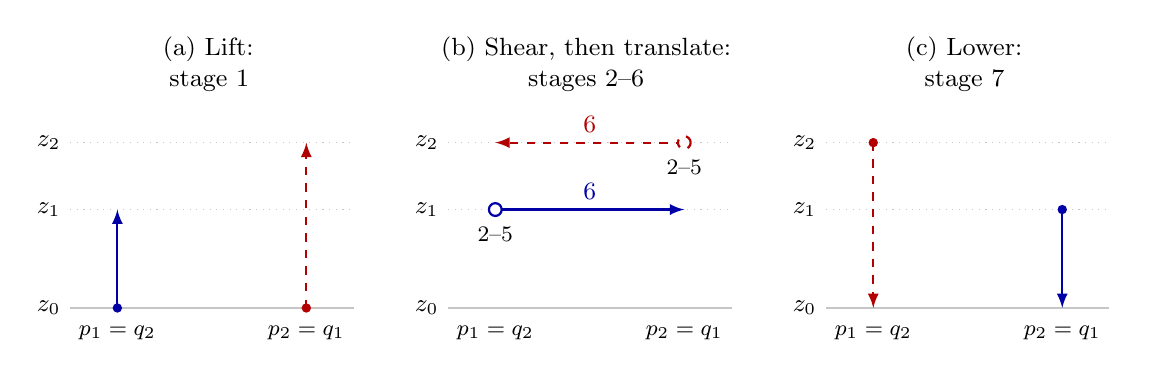
\begin{tikzpicture}[
  x=1cm,y=1cm,>=latex,
  every node/.style={font=\small},
  level/.style={gray!45,thin},
  first/.style={blue!65!black,thick},
  second/.style={red!70!black,thick,dashed}]
  \foreach \shift in {0,4.8,9.6} {
    \begin{scope}[xshift=\shift cm]
      \draw[level] (0.45,0.45)--(4.05,0.45);
      \draw[level,dotted] (0.45,1.7)--(4.05,1.7);
      \draw[level,dotted] (0.45,2.55)--(4.05,2.55);
      \node[left] at (0.45,0.45) {$z_0$};
      \node[left] at (0.45,1.7) {$z_1$};
      \node[left] at (0.45,2.55) {$z_2$};
      \node[below,font=\footnotesize] at (1.05,0.35) {$p_1=q_2$};
      \node[below,font=\footnotesize] at (3.45,0.35) {$p_2=q_1$};
    \end{scope}
  }
  \begin{scope}
    \node[align=center,text width=4.2cm] at (2.2,3.55)
      {(a) Lift:\\stage 1};
    \draw[first,->] (1.05,0.45)--(1.05,1.7);
    \draw[second,->] (3.45,0.45)--(3.45,2.55);
    \fill[blue!65!black] (1.05,0.45) circle (1.7pt);
    \fill[red!70!black] (3.45,0.45) circle (1.7pt);
  \end{scope}
  \begin{scope}[xshift=4.8cm]
    \node[align=center,text width=4.2cm] at (2.2,3.55)
      {(b) Shear, then translate:\\stages 2--6};
    \draw[first,->] (1.05,1.7)--node[above] {6}(3.45,1.7);
    \draw[second,->] (3.45,2.55)--node[above] {6}(1.05,2.55);
    \draw[first,fill=white] (1.05,1.7) circle (2.3pt);
    \draw[second,fill=white] (3.45,2.55) circle (2.3pt);
    \node[below,font=\footnotesize] at (1.05,1.6) {2--5};
    \node[below,font=\footnotesize] at (3.45,2.45) {2--5};
  \end{scope}
  \begin{scope}[xshift=9.6cm]
    \node[align=center,text width=4.2cm] at (2.2,3.55)
      {(c) Lower:\\stage 7};
    \draw[first,->] (3.45,1.7)--(3.45,0.45);
    \draw[second,->] (1.05,2.55)--(1.05,0.45);
    \fill[blue!65!black] (3.45,1.7) circle (1.7pt);
    \fill[red!70!black] (1.05,2.55) circle (1.7pt);
  \end{scope}
\end{tikzpicture}
\caption{Schematic center paths in the $x$--$z$ projection for two
branches with exchanged source and target centers; the $y$ coordinate is
suppressed. The four shears fix each center before stage 6 translates it.
Lift and lower occur at different times, so their projected overlap causes
no interference. The lines represent trajectories, not field supports.}
\label{fig:height-stages}
\end{figure}

\paragraph{Cutoffs and heights.}
For explicit smooth profiles, set
\[
 E(t)=\begin{cases}e^{-1/t},&t>0,\\0,&t\le0,\end{cases}
 \qquad S(t)=\frac{E(t)}{E(t)+E(1-t)}.
\]
Thus $S=0$ on $(-\infty,0]$ and $S=1$ on $[1,\infty)$.
For $a<b\le c<d$, the product
$S((t-a)/(b-a))S((d-t)/(d-c))$ is a cutoff supported in $[a,d]$
and equal to one on $[b,c]$. Rational choices and products of these
functions give the cutoffs below. Every product involving a chart
coordinate is supported strictly inside its chart and is extended by
zero, then periodically.

Choose rational collars around the source rectangles, pairwise disjoint
and contained in the chart. Do the same independently for the targets.
Let $\chi_i^-,\chi_i^+$ be product cutoffs supported in those collars
and equal to one on positive neighborhoods of $P_i,Q_i$. Define
\begin{equation}\label{eq:A}
 \begin{split}
 A_i^-(x,y)&=\partial_x\bigl((x-p_{i,1})\chi_i^-(x,y)\bigr),\\
 A_i^+(x,y)&=\partial_x\bigl((x-q_{i,1})\chi_i^+(x,y)\bigr).
 \end{split}
\end{equation}
Each has integral zero. It equals one near its own rectangle and zero
near every other rectangle of the same family.

Choose distinct rational heights $z_i$ in the vertical chart. Take
cutoffs $\gamma_i$ equal to one near $z_i$, with disjoint supports inside
that chart, and define
\begin{equation}\label{eq:Z}
 Z_i(z)=\partial_z\bigl((z-z_i)\gamma_i(z)\bigr).
\end{equation}
Then $\int Z_i=0$, and near $z_i$ we have $Z_i=1$ and $Z_j=0$ for
$j\ne i$. Finitely many heights leave positive rational margins. The
segment from $z_0$ to each $z_i$ stays in the chart.

Choose one-dimensional cutoffs $\rho_x,\rho_y$ equal to one on
neighborhoods of the coordinate projections of $K+[-2h,2h]^2$, with
supports inside the corresponding chart intervals. Put
\[
 g_i^x(x)=\rho_x(x)(x-p_{i,1}),\qquad
 g_i^y(y)=\rho_y(y)(y-p_{i,2}).
\]
These functions need not have zero integral: the factor $Z_i$ will supply
zero mean to their three-dimensional fields.

\paragraph{Seven fields.}
With $e_x,e_y,e_z$ the coordinate unit vectors, define
\begin{align}
 W_1&=e_z\sum_i(z_i-z_0)A_i^-, &
 W_2&=e_y\sum_i(-\lambda_i)Z_i g_i^x,\notag\\
 W_3&=e_x\sum_i(\lambda_i^{-1}-1)Z_i g_i^y, &
 W_4&=e_y\sum_i Z_i g_i^x,\notag\\
 W_5&=e_x\sum_i(\lambda_i-1)Z_i g_i^y, &
 W_6&=\sum_i Z_i\,(q_i-p_i,0),\notag\\
 W_7&=e_z\sum_i(z_0-z_i)A_i^+.&&\label{eq:fields}
\end{align}
Choose seven successive, disjoint closed intervals inside $(0,1)$ with
rational endpoints. A rescaled derivative of $S$ gives a nonnegative
smooth pulse $b_j$ of integral one in each interval. Set
\begin{equation}\label{eq:velocity}
 V(t,X)=\sum_{j=1}^7 b_j(t)W_j(X),\qquad 0\le t\le1,
\end{equation}
and extend it periodically. The pulses vanish to all orders at their
endpoints. The gaps between stages and around the ends of the period
make this extension smooth and give $V=0$ near every integer time.

\paragraph{Exact trajectories.}
Start at $(X,z_0)$ with $X\in P_i$. During the first stage its horizontal
coordinate stays fixed. Its source mask is one and every other source
mask vanishes. Integrating $b_1$ therefore lifts it exactly to $z_i$.

During the next five stages the height is fixed at $z_i$, where only
its own height mask contributes. Write $X=p_i+(r,s)$. The endpoint
half-width assumptions give
\[
 |r|,\ |s|,\ |\lambda_i r|,\ |s/\lambda_i|\le h.
\]
Lemma~\ref{lem:excursion} shows that the proposed four-shear path stays
inside $p_i+[-2h,2h]^2$. Consequently both horizontal cutoffs are one
all along it. The proposed path solves the ODE for the localized fields,
so uniqueness of the smooth ODE identifies it with the actual path.
Its endpoint is
\[
 p_i+\diag(\lambda_i,\lambda_i^{-1})(X-p_i).
\]
This argument verifies the plateau condition rather than assuming it.

The sixth field translates by $q_i-p_i$. Its path has the form in (d),
with the final offsets bounded by $h$. Convexity of $K$ keeps it in the
chart. The endpoint is $F_i(X)\in Q_i$, where the target mask is one
and all other target masks vanish. The seventh field therefore lowers
it to $z_0$. Source--target intersections cause no interference: sources
and targets are used at different times, with separate heights between.

We have proved the exact action on closed rectangles. We now give a
quantitative neighborhood argument. Each planar partial composition on a
branch is affine. Let $C\ge1$ bound the infinity operator norms of all its
linear parts, including the final composition. During a partial shear its
matrix entries depend affinely on the accumulated pulse mass; the matrix
norm is therefore bounded by the larger endpoint norm. Thus finitely many
rational matrix bounds provide $C$.

Choose positive rational margins inside the source-mask and target-mask
plateaus, the horizontal $\rho_x,\rho_y$ plateaus around all the compact
planar paths, the private height plateaus, and the vertical chart around
each lift and lowering segment. Call the respective minima
$\eta_-,\eta_+,\eta_\rho,\eta_z,\eta_{\rm chart}$.
Every minimum is positive by the chosen collars and the finite explicit
paths. Take
\[
 0<\delta<\frac12\min\{
 \eta_-,\eta_+/C,\eta_\rho/C,\eta_z,\eta_{\rm chart}\}.
\]
Starting within sup distance $\delta$ of $P_i\times\{z_0\}$, the first
mask is exactly one and all other source masks are zero. It lifts the
height from $z_0+\zeta$ to $z_i+\zeta$. This height lies in the plateau
where $Z_i=1$ and all other $Z_j=0$, including their compensating lobes.
Inductively through the planar stages, the proposed affine displacement
from a reference path is at most $C\delta$. It stays inside the horizontal
plateaus, so the affine candidate solves the actual localized ODE at every
stage. At the final planar endpoint it lies in the target-mask plateau,
where lowering sends $z_i+\zeta$ exactly to $z_0+\zeta$. ODE uniqueness
identifies these explicit candidates with the actual trajectories. This
proves the claimed map on a positive neighborhood. The radius may depend
on $\lambda_i$; the $2h$ bound on the original closed rectangles does not.

\paragraph{The equation and uniqueness.}
For $W_1,W_7$, the sole component is vertical and independent of height.
For $W_2,\ldots,W_5$, the sole component is independent of its direction
of motion. For $W_6$, both horizontal components depend only on height.
Thus each $W_j$ is divergence free and has zero self-advection. The
derivative representations \eqref{eq:A} and \eqref{eq:Z} give zero
spatial mean. Since at most one pulse is active at a time, these three
identities hold for $V$ as well; no cross-stage convection terms occur.
It follows that $f=V_t-\nu\Delta V$ is solenoidal and mean zero and
that $(V,0)$ solves \eqref{eq:NS} with zero initial velocity.

We prove uniqueness by energy comparison, as in Leray's analysis of
regular solutions~\cite[Section~18]{Leray}; the periodic forced
calculation is included here. For another solution $v$ in the stated
classical class, put $w=v-V$.
Subtract the equations and integrate by parts on the torus. The pressure
term and transport by $v$ vanish, giving
\[
 \frac12\frac{d}{dt}\|w\|_2^2+\nu\|\nabla w\|_2^2
 \le \|\nabla V\|_{\infty,\mathrm{op}}\|w\|_2^2.
\]
The stated regularity justifies these operations on each finite closed
time cylinder. Since $w(0)=0$, Gronwall's inequality gives $w=0$.
The remaining pressure gradient vanishes, and the mean-zero pressure
normalization gives $p=0$. Smooth periodicity gives uniformly bounded
kinetic energy and all derivative bounds. The smooth bounded velocity
and spatial derivative also give a unique global material flow.

\paragraph{Effective choices and evaluation.}
All rectangle gaps and chart margins are rational positive numbers.
The preceding lists, heights, collars, and pulse intervals can
therefore be chosen by finite rational calculations. On $t>0$, each
derivative of $E$ has the form $P(1/t)e^{-1/t}$ for an effectively
computable polynomial $P$. The inequalities
$e^y\ge y^m/m!$ give effective errors near zero, and
$E(t)+E(1-t)\ge e^{-2}$. Products and quotients consequently yield
effective bounds and evaluations for every derivative of each profile.
These estimates work even when an input real cannot be distinguished
from a cutoff endpoint. For periodic evaluation use a finite superset
of neighboring translates and their zero collars. Thus evaluation
requires no exact equality test on a supplied real. The same finite
construction computes every mixed derivative bound for $V$ and, from
the given computable $\nu$, for $f$.
\end{proof}

\subsection{Observation bounds}
An observation set must be avoided throughout the motion, not only
at integer samples. The endpoint-size estimate supplies this additional
information without a new transport construction.

\begin{corollary}\label{cor:observer}
Under Theorem~\ref{thm:shears}, suppose a branch satisfies
$p_{i,1},q_{i,1}\le a$. Every point starting in $P_i\times\{z_0\}$
has first coordinate at most $a+2h$ throughout the period. If instead
both centers are at least $a$, its first coordinate is at least $a-2h$.
If $\mathcal O\subseteq\T_L^3$ is open and
$Q_i\times\{z_0\}\subseteq\mathcal O$, every point starting in
$P_i\times\{z_0\}$ reaches $\mathcal O$ at the integer sample and
remains there for a time interval.
\end{corollary}
\begin{proof}
Lifting preserves the source coordinate. The four scaling stages stay
within $2h$ of $p_i$. Translation interpolates between $p_i$ and $q_i$
with an offset of size at most $h$, and lowering preserves the target
coordinate. These bounds give both inequalities. At the endpoint the
particle is in the target rectangle, and the velocity vanishes on a
neighborhood of the integer time.
\end{proof}



\section{Closed rectangles, initialization, and the all-time event}\label{sec:bridge}
We now connect the recorder to the geometric theorem. Symbolic injectivity
does not replace separation of filled rectangles: we will write down and
compare the image intervals.

\subsection{An affine map for every auxiliary instruction}
We use the positional-coding viewpoint of generalized shifts
\cite[Lemma~0]{Moore}, keeping the entire prefix intervals rather than only
their coded subsets.
Let $\mathcal A=\Sigma\times\mathcal G\times\{0,1\}$ be the complete
alphabet of Lemma~\ref{lem:recorder}, and let $m=|\mathcal A|$.
Give its symbols distinct odd digits $d_a\in\{1,3,\ldots,2m-1\}$ and set
$B=2m+1$. Define
\[
 C(a_0a_1\cdots)=\sum_{j\ge0}d_{a_j}B^{-j-1},\quad
 T_a(v)=\frac{d_a+v}{B},\quad I_a=T_a([0,1]).
\]
A code lies in its first-symbol interval, and $T_a^{-1}$ removes that
symbol. Distinct $I_a$ have gaps at least $1/B$. Distinct two-symbol
intervals $T_a(I_b)$ have gaps at least $1/B^2$: if their first symbols
differ they lie in separated first-symbol intervals; otherwise the common
map $T_a$ scales a first-symbol gap by $1/B$. These assertions concern
entire closed intervals, including their endpoints.

If the current head is at $k$, put
$L=C(s_{k-1}s_{k-2}\cdots)$ and $R=C(s_ks_{k+1}\cdots)$.
For each allowed recorder instruction
$(s,a)\mapsto(s',b,d)$, and each possible letter $l$ immediately to the
left, use the source rectangle $I_l\times I_a$. On that rectangle the
normalized update is
\begin{equation}\label{eq:b-radix-table}
\begin{array}{c|c|c}
 d&(L',R')&\text{full target rectangle}\\\hline
 +1&(T_b(L),T_a^{-1}(R))&T_b(I_l)\times[0,1]\\
 0&(L,T_b(T_a^{-1}(R)))&I_l\times I_b\\
 -1&(T_l^{-1}(L),T_l(T_b(T_a^{-1}(R))))
       &[0,1]\times T_l(I_b).
\end{array}
\end{equation}
For a right move the written letter is prefixed to the old left stack,
and the current letter is removed from the right stack. For a left move,
the old left letter is removed from the left stack and the pair $l,b$ is
prefixed to the old right tail. These descriptions prove the formulas on
coded points. The displayed affine formulas define the update on every
point of the full source rectangle and give exactly the displayed full
image. Their linear part is $\diag(B^{-d},B^d)$.

Let $\mathcal S$ be the finite recorder control set and $N=|\mathcal S|$.
Only $S_q$ with $q\in H$ are terminal controls. In particular $F_q$ and
$L_q$ are nonterminal even when $q\in H$: recording and returning must
finish before the terminal checkpoint. Put $\kappa=1/(32N)$ and
$y_0=3/8$. Enumerate the nonterminal controls and place their state squares
at
\[
 [c_s,c_s+\kappa]\times[y_0,y_0+\kappa],
 \qquad c_s=1/8+2j\kappa\quad(0\le j<N).
\]
Enumerate the terminal controls separately with
$c_s=3/4+2j\kappa$. Only as many indices as occur are used in each list.
All nonterminal squares lie in $1/8\le x<3/16$, all terminal squares
in $3/4\le x<13/16$, and distinct squares have horizontal gaps at least
$\kappa$. The physical code is
\begin{equation}\label{eq:b-code}
 G_s(L,R)=(c_s+\kappa L,y_0+\kappa R).
\end{equation}
For branch $i=(s,a,l)$, denote its source by
$P_i=G_s(I_l\times I_a)$, and its target by $Q_i$, obtained by applying
the appropriate row of \eqref{eq:b-radix-table} and then $G_{s'}$.
Thus its physical map is
\[
 F_i=G_{s'}\circ F_i^{\rm norm}\circ G_s^{-1},\qquad
 DF_i=\diag(\lambda_i,\lambda_i^{-1}),\qquad \lambda_i=B^{-d_i}.
\]

\begin{lemma}[Separate source and target gaps]\label{lem:b-gap}
The finite families $(P_i)$ and $(Q_i)$ are separately pairwise positively
separated, with gap at least $\kappa/B^2$ in some coordinate for every pair.
Their side lengths are positive, rational, and at most $\kappa$.
No source--target separation is asserted or needed.
\end{lemma}
\begin{proof}
Different source controls lie in different state squares. Within one
control, determinism permits at most one rule for a read letter $a$.
Distinct branches therefore differ in $a$ or in $l$, giving the source gap
$\kappa/B$.

For targets, different destination controls again give the state-square
gap. For one fixed destination control, Lemma~\ref{lem:recorder} gives a
single incoming displacement $d$. The same lemma says that a written
complete letter $b$ determines the preceding control and read complete
letter. Consequently two different branches entering that control must
differ in $b$ or in $l$. For $d=+1$, the left image has the two-symbol
prefix $(b,l)$; for $d=-1$, the right image has prefix $(l,b)$. The
previous two-symbol estimate gives gap $\kappa/B^2$. For $d=0$, the two
coordinates expose $l$ and $b$ separately, giving gap $\kappa/B$.
The full target descriptions in \eqref{eq:b-radix-table} prove this for
filled rectangles, not only for their tape-code subsets. The side-length
claim follows directly from those descriptions.
\end{proof}

Take $h=\kappa/2$, $z_0=1/2$, and
$K=[1/8,13/16]\times[3/8,7/16]$. Use planar charts
$(1/32,31/32)$ in both coordinates and vertical chart $(1/8,7/8)$.
Each has length strictly less than one.
All source and target centers belong to $K$, and
$K+[-2h,2h]^2$ lies strictly inside that chart. Theorem~\ref{thm:shears}
therefore produces a period-one velocity $V_M$ acting exactly on all these
rectangles and on positive neighborhoods of them. This construction uses
only the finite recorder table and rational choices; it does not depend on
which branches will be visited.

For every branch with nonterminal source and target, both first-coordinate
centers are at most $1/4$. Corollary~\ref{cor:observer} then gives throughout
its entire period
\begin{equation}\label{eq:b-safe}
 x\le1/4+2h=1/4+\kappa\le9/32<1/2.
\end{equation}
Every terminal code has $x\ge3/4$ and hence lies in $O$.
The estimate \eqref{eq:b-safe} is deliberately applied only to branches
whose two ends are nonterminal; the last transition into a terminal
checkpoint may enter the detector. No identity rule is added at terminal
controls. Such a rule could conflict with an incoming target and is
unnecessary for a reachability assertion.

\subsection{Loading the fixed label}
Initialize the recorder at head zero and control $S_{q_0}$, with the original
finite work input, frontier $P$ at cell $2$, history $E$ at every other
cell, and every return mark zero. Both complete tape tails are eventually
the constant symbol $(\square,E,0)$. If a tail is constant after $r$ symbols,
its code equals a finite rational sum plus
$B^{-r}d_{(\square,E,0)}/(B-1)$. Hence its initial physical point
$P_{\rm in}=(x_{\rm in},y_{\rm in})$ is computed by finite rational
arithmetic, including all history and mark tracks.

Choose a smooth periodic function $Z$ with zero integral and $Z=1$ near
$z_0=1/2$, for example
$Z(z)=\partial_z((z-z_0)\gamma(z))$ with $\gamma=1$ near $z_0$ and
supported strictly inside $(0,1)$. Choose nonnegative smooth pulses
$\beta_x,\beta_y$ of integral one, supported respectively in
$(1/8,3/8)$ and $(5/8,7/8)$. Define on $0\le t\le1$
\begin{equation}\label{eq:b-loader}
 U_{\rm load}(t,x,y,z)=
 \beta_x(t)(x_{\rm in}-1/8)Z(z)e_x+
 \beta_y(t)(y_{\rm in}-3/8)Z(z)e_y.
\end{equation}
The point $a_*$ first travels horizontally from $(1/8,3/8,z_0)$ to
$(x_{\rm in},3/8,z_0)$, then vertically in the planar chart to
$(x_{\rm in},y_{\rm in},z_0)$. Height stays $z_0$, so $Z=1$ along both
segments. If the initial control is nonterminal, this path stays in
$x\le1/4$. If it is terminal, the endpoint is already in $O$, as required.
Both velocity terms have zero spatial mean and zero self-advection, and their
supports in time are disjoint.

Now prescribe
\begin{equation}\label{eq:b-U}
 U(t)=\begin{cases}U_{\rm load}(t),&0\le t\le1,\\
                    V_M(t-1),&t\ge1.
       \end{cases}
\end{equation}
Both pieces vanish on neighborhoods of their joining time. The field is
therefore smooth, starts at zero, and has period one after time one.
Every derivative is globally bounded: the loader is a finite collection
of smooth profiles on a compact interval, and the remaining mechanism
is smooth and periodic. Its mean, divergence, and self-advection all
vanish at every time.

\subsection{Completion of the fluid and observation statements}
After loading, the particle is precisely the initial code at height $z_0$.
At every initialized microstep before a terminal checkpoint it belongs to
one and only one source rectangle: its control and the two first letters select that
branch. Equations \eqref{eq:b-radix-table} and \eqref{eq:b-code}, together
with Theorem~\ref{thm:shears}, send it to exactly the successor recorder
code at height $z_0$. This proves the simulation by induction over all
microsteps that are defined. The checkpoint induction in
Lemma~\ref{lem:recorder} verifies every guard between these checkpoints;
arbitrary malformed nonterminal tapes are not asserted to have successors.

If the original machine never halts, Lemma~\ref{lem:recorder} says that
all recorder steps are defined. It also says that each original instruction
finishes after the positive finite number
$2(2+n-h_{n+1})+4$ of microsteps. In fact this is at least $6$, since
$h_{n+1}\le n+1$. Thus the nonhalting run yields infinitely many periods;
no accumulation of infinitely many periods in finite time occurs. All
control states encountered are nonterminal, so \eqref{eq:b-safe} excludes
$O$ at every intermediate time, while the loader is safe by construction.

If the machine halts after finitely many original instructions, the finite
sum of their finite microstep counts gives a finite period at which the
particle reaches a terminal checkpoint, whose code belongs to $O$.
If it was initially halted, the loader supplies the hit. A machine with
no original instruction at a nonhalting pair is first normalized by the
explicit stationary stop transition in Section~\ref{sec:recorder}; if its
initial state is already halting, only the loader is needed for the hit. We impose no
condition on later motion after a hit. This proves both directions of
the event equivalence for all real times.

Finally set
\begin{equation}\label{eq:b-force}
 f_{M,w}=U_t-\nu\Delta U.
\end{equation}
Since $(U\cdot\nabla)U=0$, substitution proves that $(U,0)$ solves
\eqref{eq:NS}. Differentiation and integration preserve the vanishing
divergence and mean, so the force is solenoidal and mean zero. Its
smoothness, periodicity after initialization, and mixed-derivative bounds
follow from those of $U$. The energy comparison proved in
Theorem~\ref{thm:shears} applies on every finite interval also across
initialization: the reference gradient is bounded there and no time
symmetry is required of a competitor. It gives uniqueness in the stated
class. Compactness of the torus and the uniform bound for $U$ give the
uniform energy bound and the global material flow.

All state placements, digits, rectangles, and initial rational codes are
finite constructions. The effective cutoffs and pulses were proved in
Theorem~\ref{thm:shears}; the one-time loader uses the same profiles.
An approximate time argument near the join may be handled by evaluating
both smooth terms using their zero collars. Periodic evaluation uses a
finite superset of nearby translates. Thus no exact equality test at a
joining time is needed, and no part of the force evaluator follows the
particular machine execution. This completes
Theorem~\ref{thm:initialized}.

The loader accounts for the time qualification in that theorem. Periodicity
from time zero would require a repeated initialization rule or an
input-dependent placement inside the periodic mechanism; it does not follow
from adding a one-time loader. The present theorem asserts periodicity after initialization.

\begin{corollary}[Undecidability of the fixed particle event]
No algorithm decides the event of Theorem~\ref{thm:initialized} for every
finite force prescription produced by its compiler.
\end{corollary}
\begin{proof}
Such an algorithm, composed with the terminating force compiler, would
decide halting for arbitrary finite machine descriptions and inputs. It would
also decide Turing's symbol-printing problem \cite[Section~8]{Turing}: modify
a machine to halt upon printing the specified symbol and to run forever
otherwise, including when it stops without printing that symbol. Turing's
undecidability theorem excludes this algorithm.
\end{proof}

\section{Optional recorder and schedule changes}\label{sec:optional}
The complete initialized construction above uses neither of the changes
in this section. They record two ways to adapt its finite mechanism while
retaining the stated inverse and geometric bounds.

\subsection{Keeping the return mark at checkpoints}
Some encodings use a marked work head at a checkpoint. This change has an
exact description on all configurations, so it does not require a separate
simulation argument.

Let $T$ be the partial transition of Lemma~\ref{lem:recorder}. Define an
involution $J$ on recorder configurations by toggling the mark under the
head when the control is $S_q$, and making no change in any other control.
The head position, control, work track, and history track remain fixed. Put
\begin{equation}\label{eq:conjugacy}
 T_{\mathrm{per}}=J\circ T\circ J,
 \qquad \operatorname{dom}T_{\mathrm{per}}=J(\operatorname{dom}T).
\end{equation}
Only the first and last rows of the table change. The first now reads mark
one and writes mark zero before moving to $A_r$. The last preserves mark
one while entering $S_q$. All five other rows, including their history
guards, are unchanged.

Because $J^2=\id$, the identity
$T_{\mathrm{per}}^k=J T^k J$ holds wherever either corresponding iterate
is defined. Initialize with the sole mark at the work head. The conjugacy
then transfers the checkpoint invariant, the step count, and halting
equivalence from Lemma~\ref{lem:recorder}. Its two incoming properties also
hold directly: at $A_r$ the old mark is known to be one, and at $S_q$ the
last row copies the marked symbol. Every other inverse is unchanged.
This is an equality of partial maps, not just an equivalence of initialized
runs.

One may also adjoin a passive track with any finite alphabet. Extend every
rule over every value of that track and preserve it at each write. The
inverse above reconstructs the active tracks, while the written passive
value reconstructs itself. Thus both incoming properties and the checkpoint
proof persist. In particular, a passive track initially marked only at the
origin retains an absolute reference position. This extension does not
change any history guard or append rule.

\subsection{Alternative shear schedules}
\begin{remark}[Two schedule variants]\label{rem:variants}
The chronological list
\[
 \mathsf X(\lambda^{-1}-1),\quad \mathsf Y(1),\quad
 \mathsf X(\lambda-1),\quad \mathsf Y(-\lambda^{-1})
\]
has the successive endpoints
\begin{align*}
 &(r+(\lambda^{-1}-1)s,s),\\
 &(r+(\lambda^{-1}-1)s,r+s/\lambda),\\
 &(\lambda r,r+s/\lambda),\\
 &(\lambda r,s/\lambda).
\end{align*}
The proof of Lemma~\ref{lem:excursion} bounds each coordinate by $2h$;
convexity handles partial shears. Replacing the four middle scaling
fields accordingly preserves the rest of Theorem~\ref{thm:shears}.

Alternatively, split $W_6$ into its two horizontal components and give
them successive unit-integral pulses. This gives eight stages with
one Cartesian component active at a time. The horizontal center now
moves first in one coordinate and then in the other. Both segments
stay in the rectangle $K$, so the coordinate bounds and the proof of
Corollary~\ref{cor:observer} persist. Every field is still transverse,
mean zero, and free of self-advection. This variant has the same
endpoint map, although its translation path differs.
\end{remark}

\begin{thebibliography}{9}
\addcontentsline{toc}{section}{References}
\raggedright
\bibitem{Bennett}
C.~H. Bennett,
\emph{Logical reversibility of computation},
IBM Journal of Research and Development \textbf{17} (1973), no.~6,
525--532.
\href{https://doi.org/10.1147/rd.176.0525}{doi:10.1147/rd.176.0525}.

\bibitem{CMP}
R. Cardona, E. Miranda and D. Peralta-Salas,
\emph{Computability and Beltrami fields in Euclidean space},
Journal de Math\'ematiques Pures et Appliqu\'ees \textbf{169} (2023), 50--81.
\href{https://doi.org/10.1016/j.matpur.2022.11.007}{doi:10.1016/j.matpur.2022.11.007}.

\bibitem{CMPP}
R. Cardona, E. Miranda, D. Peralta-Salas and F. Presas,
\emph{Constructing Turing complete Euler flows in dimension 3},
Proceedings of the National Academy of Sciences \textbf{118} (2021),
e2026818118.
\href{https://doi.org/10.1073/pnas.2026818118}{doi:10.1073/pnas.2026818118}.

\bibitem{DGMP}
S. Dyhr, \'A. Gonz\'alez-Prieto, E. Miranda and D. Peralta-Salas,
\emph{Turing complete Navier--Stokes steady states via cosymplectic geometry},
PNAS Nexus \textbf{5} (2026), pgag131.
\href{https://doi.org/10.1093/pnasnexus/pgag131}{doi:10.1093/pnasnexus/pgag131}.

\bibitem{Landauer}
R. Landauer,
\emph{Irreversibility and heat generation in the computing process},
IBM Journal of Research and Development \textbf{5} (1961), no.~3,
183--191.
\href{https://doi.org/10.1147/rd.53.0183}{doi:10.1147/rd.53.0183}.

\bibitem{Leray}
J. Leray,
\emph{Sur le mouvement d'un liquide visqueux emplissant l'espace},
Acta Mathematica \textbf{63} (1934), 193--248.
\href{https://doi.org/10.1007/BF02547354}{doi:10.1007/BF02547354}.

\bibitem{Moore}
C. Moore,
\emph{Generalized shifts: unpredictability and undecidability in
dynamical systems},
Nonlinearity \textbf{4} (1991), no.~2, 199--230.
\href{https://doi.org/10.1088/0951-7715/4/2/002}{doi:10.1088/0951-7715/4/2/002}.

\bibitem{Turing}
A. M. Turing, \emph{On computable numbers, with an application to the
Entscheidungsproblem}, Proceedings of the London Mathematical Society (2)
\textbf{42} (1936--1937), 230--265.
\href{https://doi.org/10.1112/plms/s2-42.1.230}{doi:10.1112/plms/s2-42.1.230}.
\end{thebibliography}
\end{document}
